\subsection{Movimento das juntas e seguimento da referência da cinemática inversa}
\label{sec:cap4_app_final_juntas}

O movimento das juntas do manipulador durante a aproximação final foi planejado de forma a posicionar a ferramenta em uma configuração adequada para o acoplamento, respeitando limites articulares e mantendo erros de seguimento reduzidos em relação à referência de cinemática inversa.
A Figura~\ref{fig:cap4_app_final_juntas} ilustra a evolução das posições, velocidades e torques nas três juntas ao longo do tempo.

\begin{figure}[H]
\centering
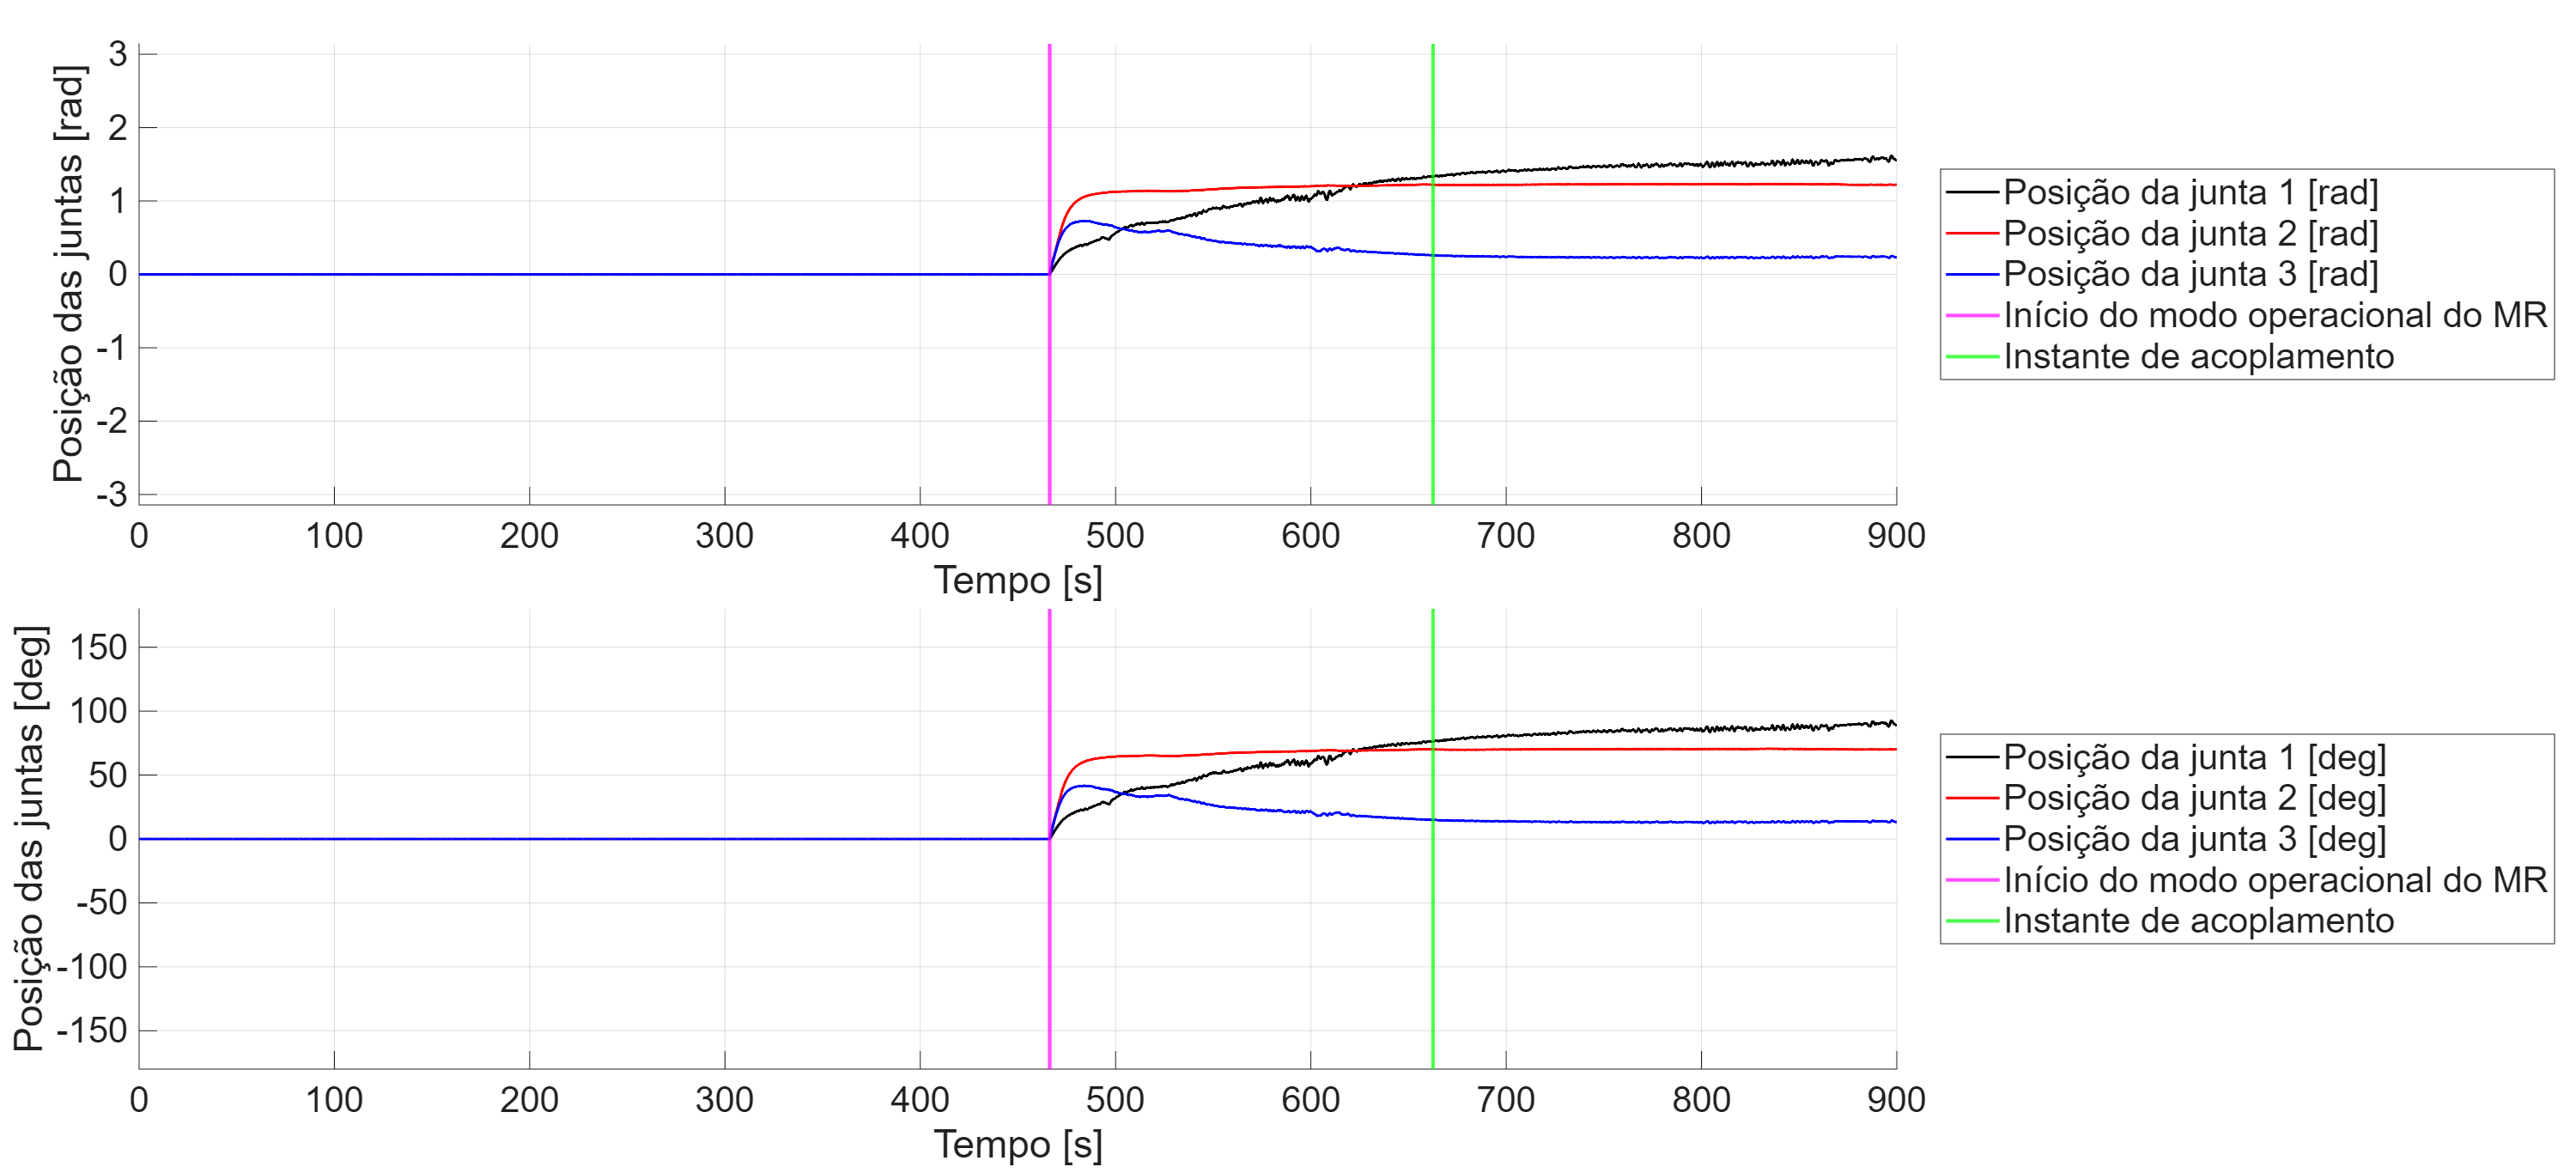
\includegraphics[width=1.0\linewidth]{4 Resultados e discussoes/Imagens/3 App final/4A Posicao velocidade e torque juntas MR.png}
\caption{Posição, velocidade e torque nas juntas do manipulador durante a aproximação final.}
\label{fig:cap4_app_final_juntas}
\end{figure}

%%%%%%%%%%%%% POSIÇÃO ARTICULAR

A Tabela~\ref{tab:cap4_juntas_pos_rad} apresenta, para cada junta do manipulador robótico, os valores mínimo e máximo observados ao longo da simulação e o valor final ao término do intervalo analisado.

\begin{table}[H]
\centering
\caption{Movimentação de cada junta do MR em radianos.}
\label{tab:cap4_juntas_pos_rad}
\begin{tabularx}{\linewidth}{|
  >{\centering\arraybackslash}X|
  >{\centering\arraybackslash}X|
  >{\centering\arraybackslash}X|}
\hline
\textbf{Junta} &
\textbf{Medição de $j_i$ ao longo da simulação [rad]} &
\textbf{Medição final $j_i$ [rad]} \\
\hhline{|=|=|=|}
$j_1$ & $0{,}00 \text{ a } 1{,}62$ & $1{,}55$ \\
\hline
$j_2$ & $0{,}00 \text{ a } 1{,}23$ & $1{,}22$ \\
\hline
$j_3$ & $0{,}00 \text{ a } 0{,}73$ & $0{,}23$ \\
\hline
\end{tabularx}
\end{table}

De forma complementar, a Tabela~\ref{tab:cap4_juntas_pos_deg} apresenta os mesmos resultados, porém em graus.

\begin{table}[H]
\centering
\caption{Movimentação de cada junta do MR em graus.}
\label{tab:cap4_juntas_pos_deg}
\begin{tabularx}{\linewidth}{|
  >{\centering\arraybackslash}X|
  >{\centering\arraybackslash}X|
  >{\centering\arraybackslash}X|}
\hline
\textbf{Junta} &
\textbf{Medição de $j_i$ ao longo da simulação [$^\circ$]} &
\textbf{Medição final $j_i$ [$^\circ$]} \\
\hhline{|=|=|=|}
$j_1$ & $0{,}00 \text{ a } 92{,}65$ & $88{,}70$ \\
\hline
$j_2$ & $0{,}00 \text{ a } 70{,}60$ & $70{,}08$ \\
\hline
$j_3$ & $0{,}00 \text{ a } 41{,}69$ & $13{,}12$ \\
\hline
\end{tabularx}
\end{table}


%%%%%%%%%%%%% VELOCIDADES ARTICULARES

\subsubsection{Velocidades das juntas}

As velocidades das juntas apresentadas na Figura~\ref{fig:cap4_app_final_velocjuntas}, permanecem de baixa magnitude ao longo de toda a fase operacional do \gls{mr}.
Observa-se que os maiores módulos ocorrem nas juntas 1 e 3, com picos de aproximadamente $0{,}26~\mathrm{rad/s}$, enquanto a junta 2 apresenta variações inferiores a $0{,}12~\mathrm{rad/s}$.

\begin{figure}[H]
\centering
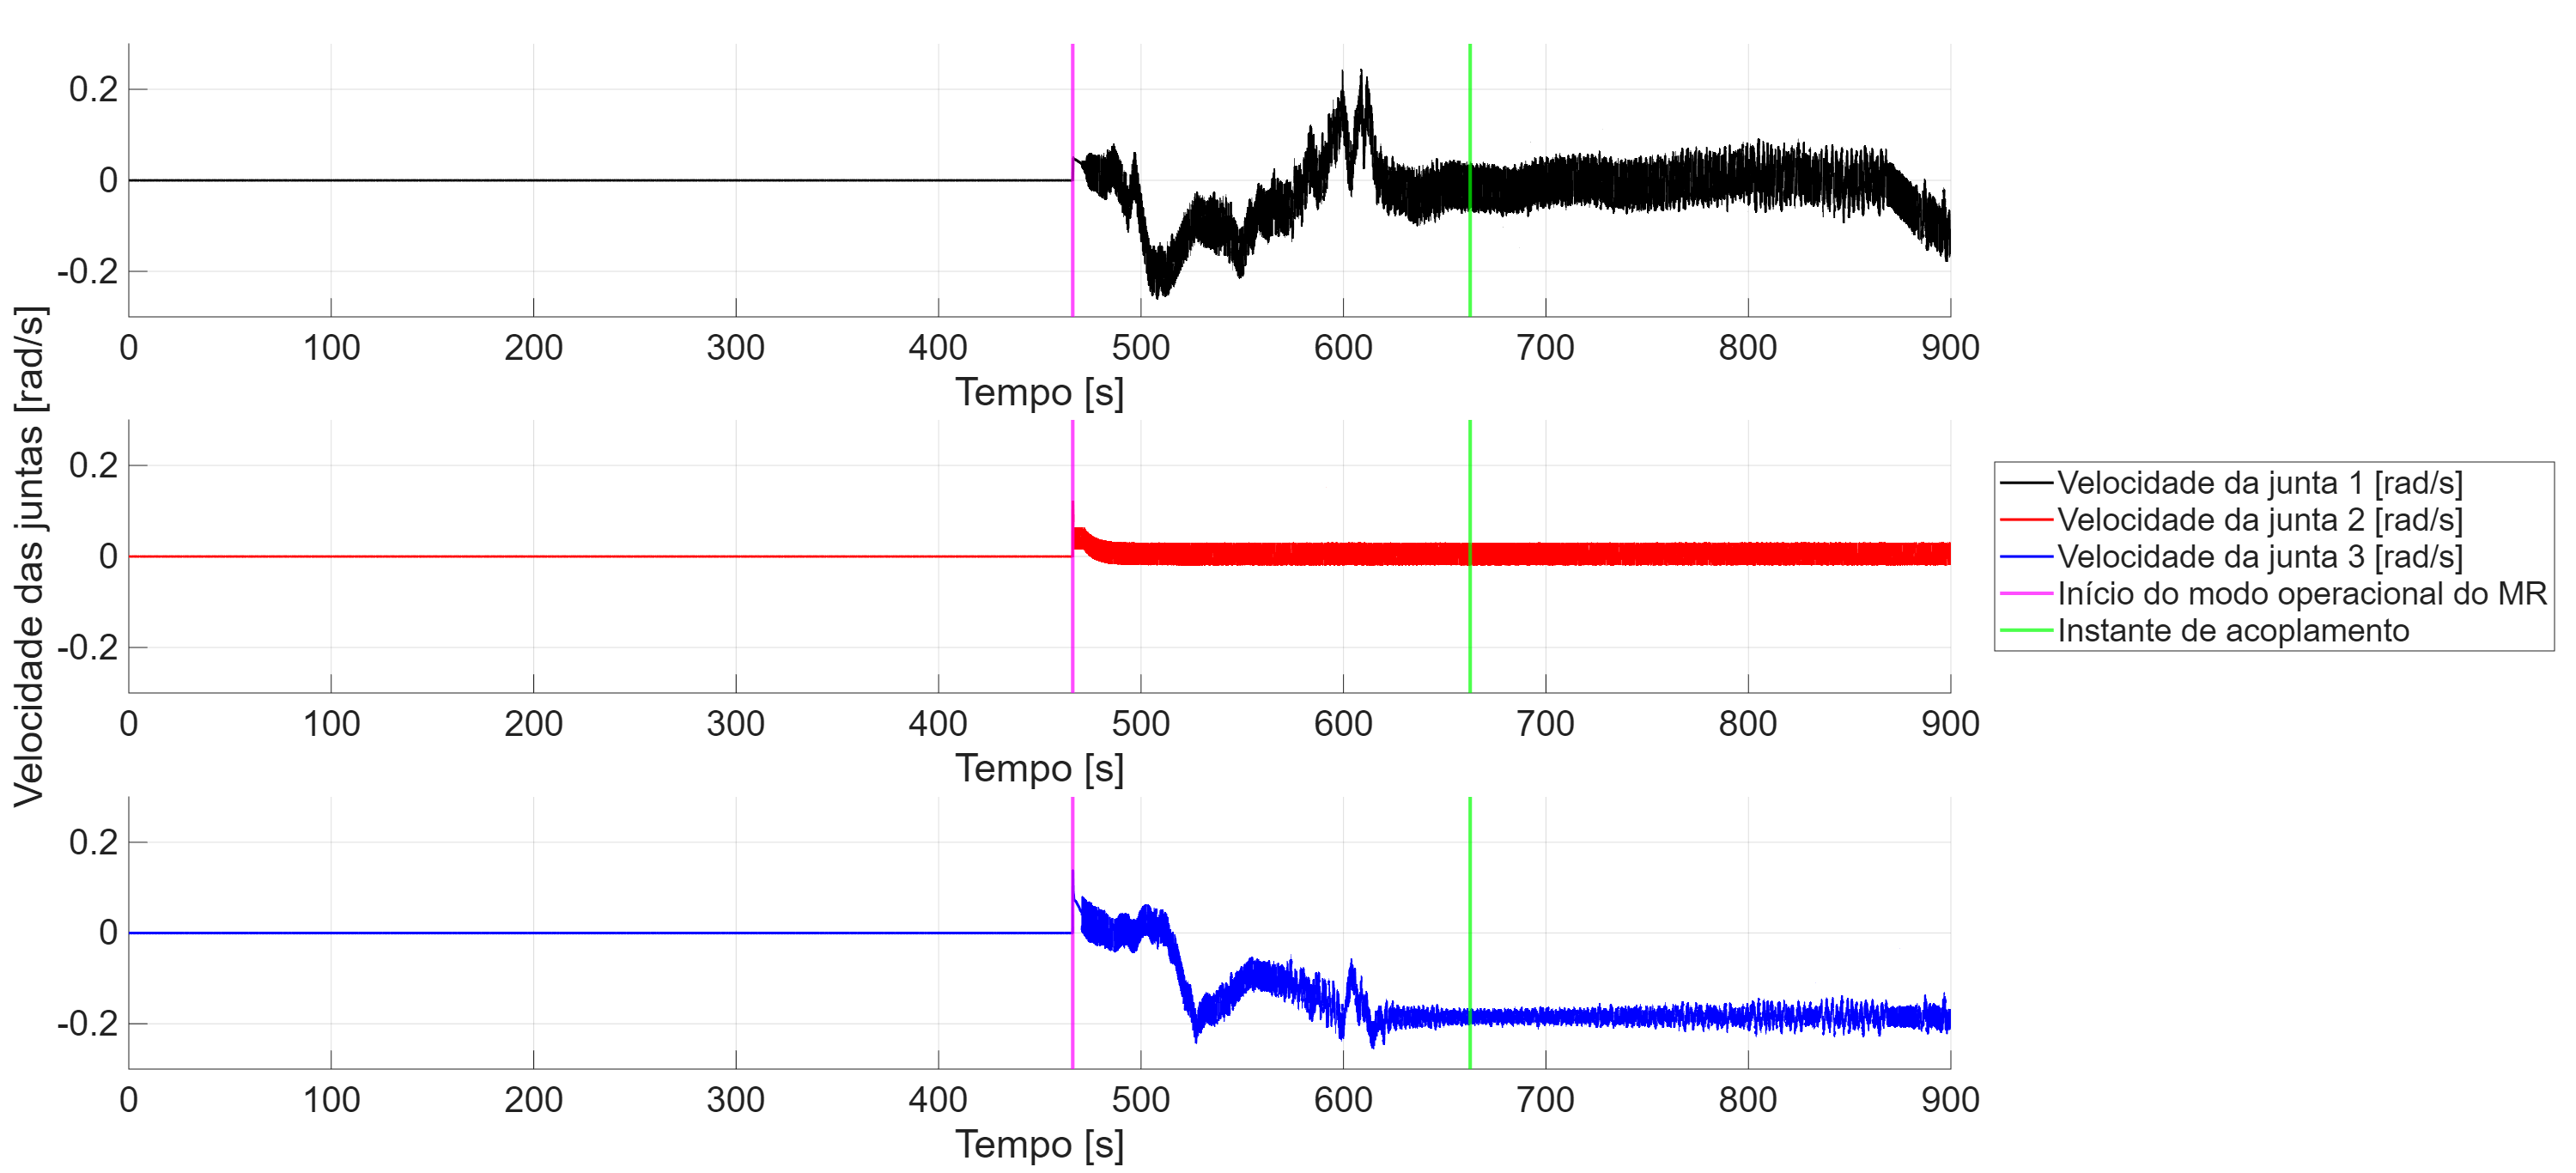
\includegraphics[width=1.0\linewidth]{4 Resultados e discussoes/Imagens/3 App final/4B Velocidade das juntas.png}
\caption{Posição, velocidade e torque nas juntas do manipulador durante a aproximação final.}
\label{fig:cap4_app_final_velocjuntas}
\end{figure}

A Tabela~\ref{tab:cap4_juntas_vel} sintetiza os valores mínimo e máximo de $\dot{j}_i$ ao longo da simulação e o valor final em rad/s.

\begin{table}[H]
\centering
\caption{Velocidades articulares em rad/s.}
\label{tab:cap4_juntas_vel}
\begin{tabularx}{\linewidth}{|
  >{\centering\arraybackslash}X|
  >{\centering\arraybackslash}X|
  >{\centering\arraybackslash}X|}
\hline
\textbf{Junta} &
\textbf{Variação de $\dot{j}_i$ ao longo da simulação [rad/s]} &
\textbf{Valor final $\dot{j}_i$ [rad/s]} \\
\hhline{|=|=|=|}
$\dot{j}_1$ & $-0{,}26 \text{ a } 0{,}24$ & $-0{,}12$ \\
\hline
$\dot{j}_2$ & $-0{,}02 \text{ a } 0{,}12$ & $0{,}01$ \\
\hline
$\dot{j}_3$ & $-0{,}25 \text{ a } 0{,}14$ & $-0{,}19$ \\
\hline
\end{tabularx}
\end{table}

A Tabela~\ref{tab:cap4_juntas_vel_deg} apresenta os mesmos resultados em graus por segundo.

\begin{table}[H]
\centering
\caption{Velocidades articulares em graus por segundo.}
\label{tab:cap4_juntas_vel_deg}
\begin{tabularx}{\linewidth}{|
  >{\centering\arraybackslash}X|
  >{\centering\arraybackslash}X|
  >{\centering\arraybackslash}X|}
\hline
\textbf{Junta} &
\textbf{Variação de $\dot{j}_i$ ao longo da simulação [$^\circ$/s]} &
\textbf{Valor final $\dot{j}_i$ [$^\circ$/s]} \\
\hhline{|=|=|=|}
$\dot{j}_1$ & $-14{,}86 \text{ a } 13{,}89$ & $-6{,}67$ \\
\hline
$\dot{j}_2$ & $-1{,}07 \text{ a } 6{,}88$ & $0{,}42$ \\
\hline
$\dot{j}_3$ & $-14{,}56 \text{ a } 7{,}89$ & $-10{,}91$ \\
\hline
\end{tabularx}
\end{table}

%%%%%%%%%%%%% TORQUE DE CONTROLE NAS JUNTAS

\subsubsection{Torque de controle nas juntas}

Os torques de controle nas juntas, apresentados na Figura~\ref{fig:cap4_app_final_torquejuntas} permanecem entre $\pm 0{,}2~\mathrm{Nm}$ ao longo de toda a fase operacional do \gls{mr}.

\begin{figure}[H]
\centering
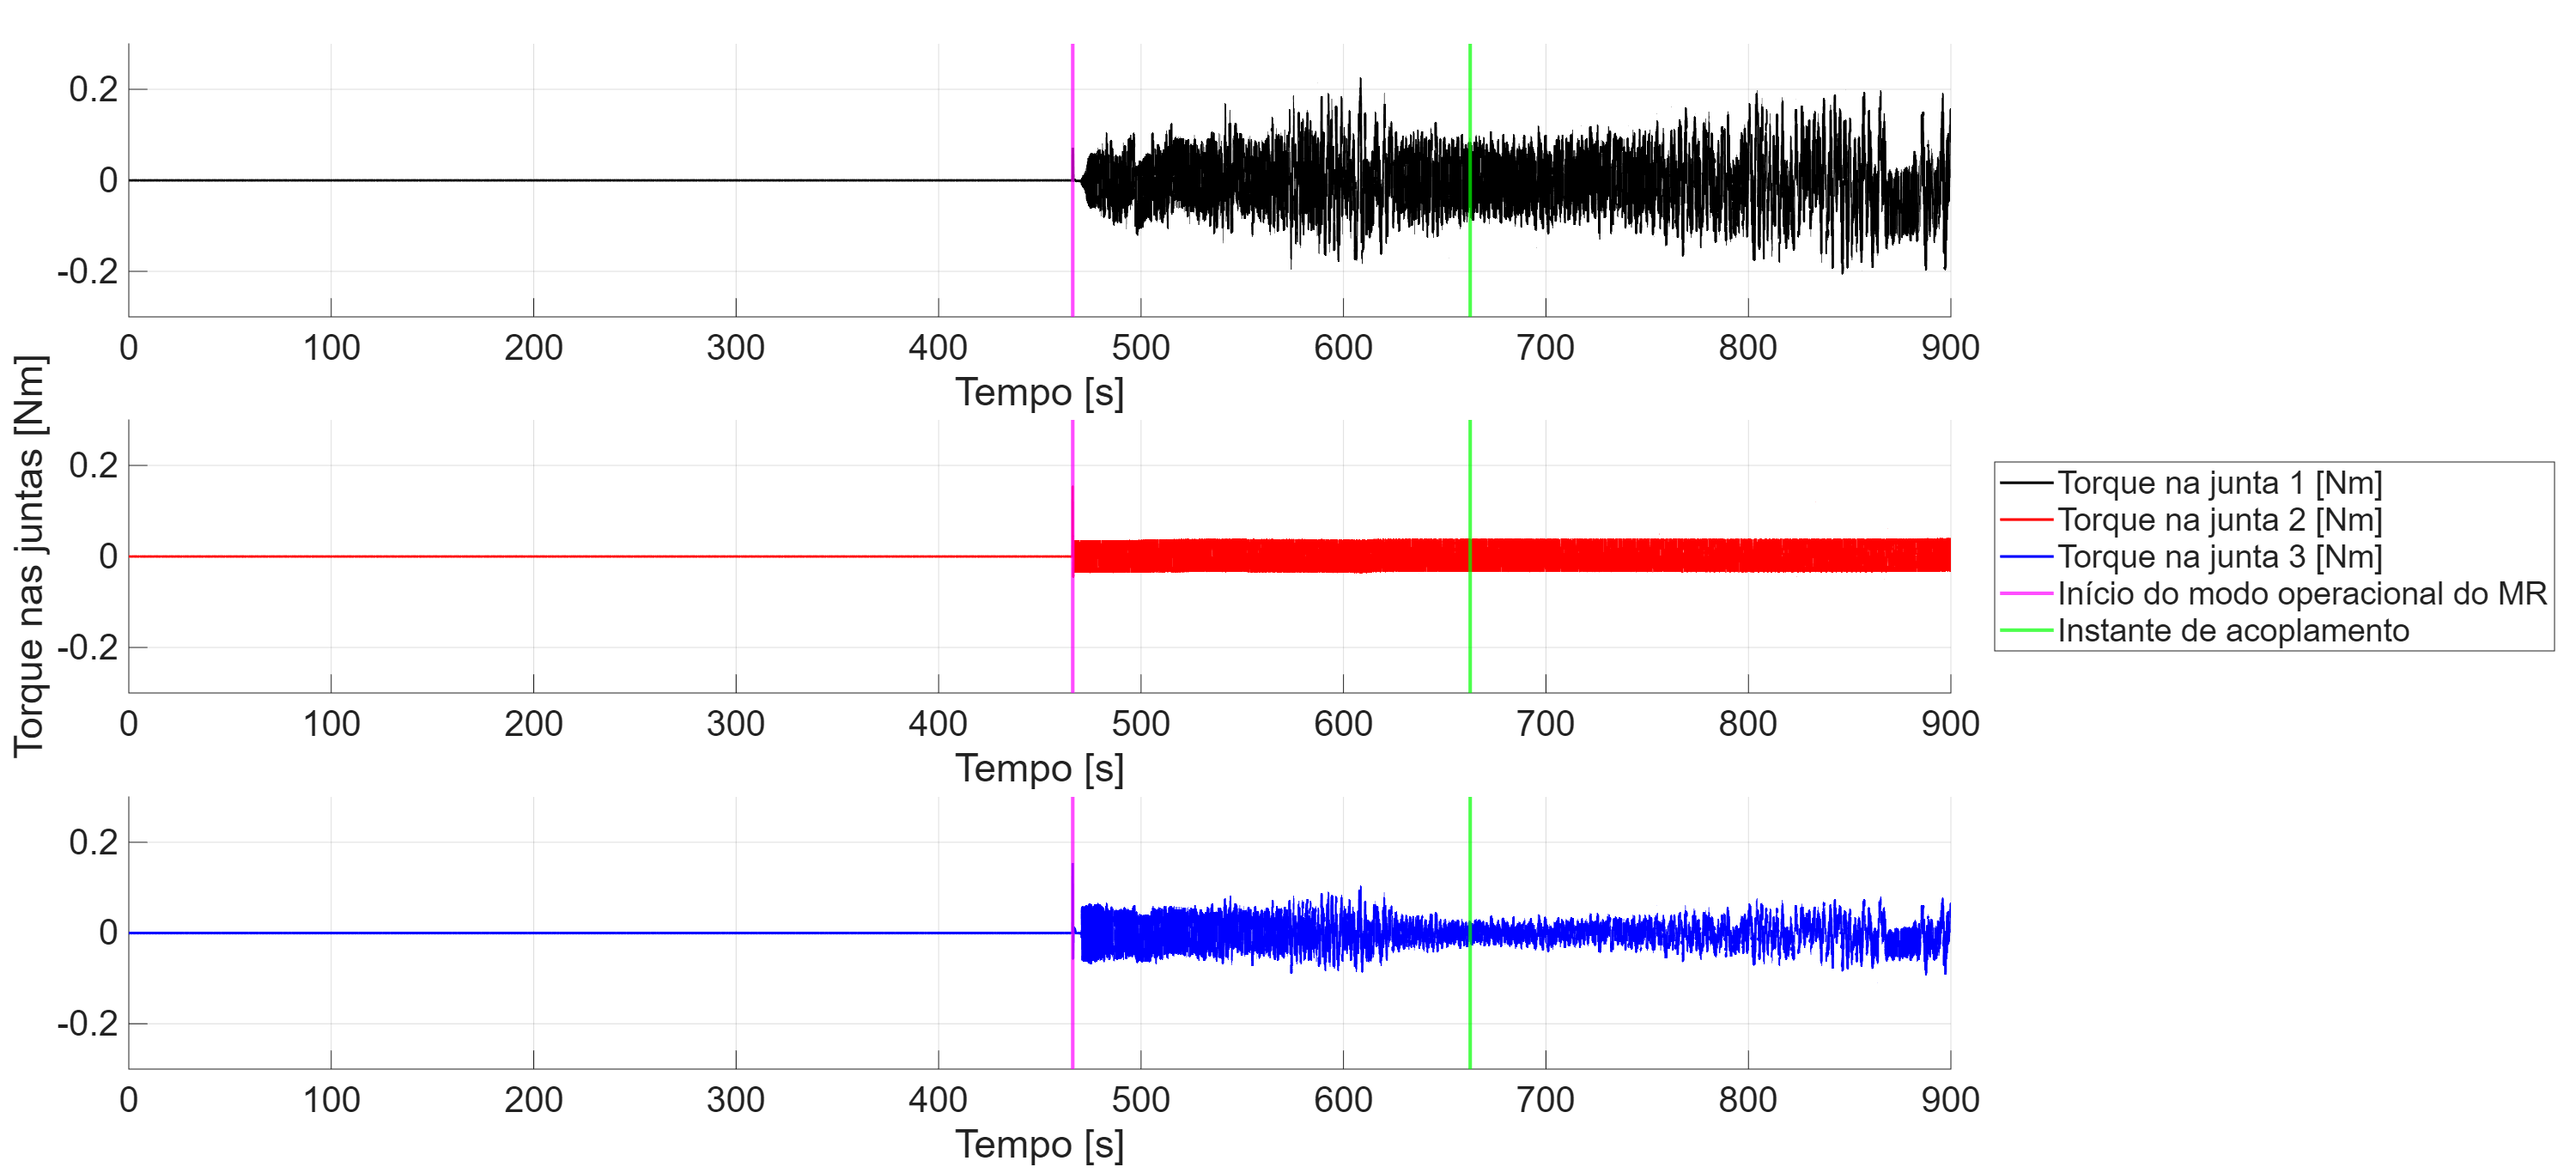
\includegraphics[width=1.0\linewidth]{4 Resultados e discussoes/Imagens/3 App final/4C Torque nas juntas.png}
\caption{Posição, velocidade e torque nas juntas do manipulador durante a aproximação final.}
\label{fig:cap4_app_final_torquejuntas}
\end{figure}

Observa-se que a junta 1 apresenta maior variação, enquanto as juntas 2 e 3 permanecem relativamente mais estáveis.
Esse comportamento observado na junta 1 acontece pois ela produz correções de orientação do conjunto do manipulador com maior efetividade para reduzir o erro de alinhamento do eixo da ferramenta com a normal da porta; possuindo menor necessidade de alterar a configuração das próximas juntas.
Portanto, o controle tende a concentrar em $j_1$ os ajustes finos de alinhamento, preservando $j_2$ e $j_3$ para compensações de menor amplitude associadas ao seguimento de posição e à manutenção da postura.
A Tabela~\ref{tab:cap4_juntas_torque} apresenta as faixas de variação e os valores finais dos torques de controle.

\begin{table}[H]
\centering
\caption{Medição dos torques de controle nas juntas.}
\label{tab:cap4_juntas_torque}
\begin{tabularx}{\linewidth}{|
  >{\centering\arraybackslash}X|
  >{\centering\arraybackslash}X|
  >{\centering\arraybackslash}X|}
\hline
\textbf{Junta} &
\textbf{Variação do torque ao longo da simulação [Nm]} &
\textbf{Medição final de torque [Nm]} \\
\hhline{|=|=|=|}
$\tau_1$ & $-0{,}20 \text{ a } 0{,}22$ & $0{,}09$ \\
\hline
$\tau_2$ & $-0{,}04 \text{ a } 0{,}15$ & $0{,}00$ \\
\hline
$\tau_3$ & $-0{,}09 \text{ a } 0{,}15$ & $0{,}04$ \\
\hline
\end{tabularx}
\end{table}


%%%%%%%%%%%%%%%%%% ERROS DE SEGUIMENTO

\subsubsection{Erro de seguimento}

A Figura~\ref{fig:cap4_app_final_erro_eef} apresenta o erro de seguimento em posição da ferramenta, definido como a diferença entre a posição de referência fornecida pela cinemática inversa (associada ao alinhamento e à aproximação da porta de acoplamento) e a posição efetivamente executada pelo efetuador final, ambas expressas no referencial ${0}$.
O segundo subgráfico corresponde a uma ampliação da escala vertical, com o objetivo de evidenciar a magnitude do erro residual, em metros, entre a posição desejada e a posição realizada.

\begin{figure}[H]
\centering

\includegraphics[width=1.0\linewidth]{4 Resultados e discussoes/Imagens/3 App final/9 Erro eef.png}
\caption{Erro de posição da ferramenta em relação à referência, expresso no frame $\{0\}$.}
\label{fig:cap4_app_final_erro_eef}
\end{figure}

A Tabela~\ref{tab:cap4_erro_pos_ferramenta} resume as faixas e os valores finais do erro de posição por componente.
Ao final da aproximação, os erros residuais permanecem da ordem de centésimos de metro, indicando convergência da trajetória executada para a referência.

\begin{table}[H]
\centering
\caption{Medição do erro de posição da ferramenta no frame $\{0\}$.}
\label{tab:cap4_erro_pos_ferramenta}
\begin{tabularx}{\linewidth}{|
  >{\centering\arraybackslash}X|
  >{\centering\arraybackslash}X|
  >{\centering\arraybackslash}X|}
\hline
\textbf{Componente} &
\textbf{Medição ao longo da simulação [m]} &
\textbf{Medição final [m]} \\
\hhline{|=|=|=|}
$e_{p,x}$ & $-0{,}25 \text{ a } 0{,}01$ & $0{,}01$ \\
\hline
$e_{p,y}$ & $-0{,}85 \text{ a } 0{,}01$ & $0{,}00$ \\
\hline
$e_{p,z}$ & $-0{,}01 \text{ a } 0{,}98$ & $-0{,}01$ \\
\hline
\end{tabularx}
\end{table}

De forma complementar, a Tabela~\ref{tab:cap4_erro_pos_ferramenta_norma} apresenta a norma do erro de posição, permanecendo inferior a $0{,}02~\mathrm{m}$.

\begin{table}[H]
\centering
\caption{Medição da norma do erro de posição da ferramenta.}
\label{tab:cap4_erro_pos_ferramenta_norma}
\begin{tabularx}{\linewidth}{|
  >{\centering\arraybackslash}X|
  >{\centering\arraybackslash}X|
  >{\centering\arraybackslash}X|}
\hline
\textbf{Grandeza} &
\textbf{Faixa ao longo da simulação [m]} &
\textbf{Valor final [m]} \\
\hhline{|=|=|=|}
$\|e_p\|$ & $0{,}00 \text{ a } 367{,}67$ & $0{,}02$ \\
\hline
\end{tabularx}
\end{table}

Por fim, conforme apresentado por Figuras e Tabelas, os resultados indicam que o manipulador robótico acompanha a referência de cinemática inversa com baixo erro residual.